\chapter{Use Cases}
\label{chapter:use cases}

\begin{wrapfigure}[11]{r}{4cm}
    \vspace{0cm}
    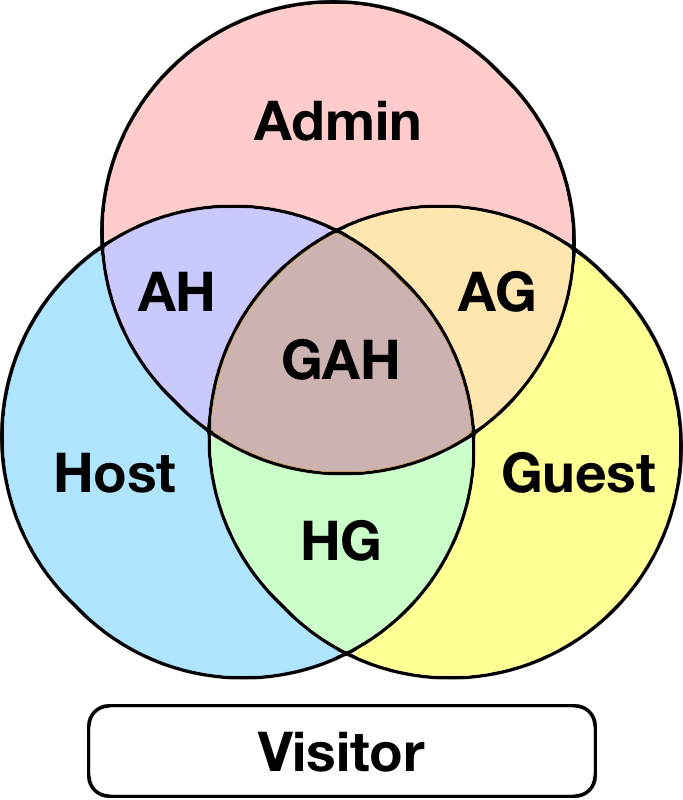
\includegraphics[width=4cm]{img/usecase_venn.png} \\[0.5em]
    \vspace{-1.2cm}
    \caption{Use Cases Actor Colour Guide}
    \label{use-case-colours}
    \end{wrapfigure} 

\section{Overview}
Surveying our functional requirements, we determined that all use cases for the System would involve the manipulation of our main entities in typical CRUD-like fashion: all the required functionality could be achieved by Creating, Viewing/Reading/Listing, Updating/Editing and Deleting these entities. Each functional requirement that did not by itself constitute any such operation (for example, filtering and ordering Properties by their Details) could be construed as forming part of some use case that did (the aforementioned filtering/ordering being subsumed under the Listing of Properties).\footnote{Refer back to Chapter \ref{chapter:requirements} for more detailed information on which requirements are covered by which use case.} Table \ref{use-cases} shows our final list of use cases, with the cells colour-coded by Primary Actor (see Figure \ref{use-case-colours} for the key to these colours). Each row of the table corresponds to one of our main entities, and the columns represent the different kinds of operations users can perform on these entities.

\definecolor{Gray}{gray}{0.9}
\definecolor{A}{rgb} {1.00,0.80,0.80}
\definecolor{H}{rgb} {0.70,0.90,1.00}
\definecolor{G}{rgb} {1.00,1.00,0.60}
\definecolor{AH}{rgb}{0.80,0.80,1.00}
\definecolor{AG}{rgb}{1.00,0.90,0.70}
\definecolor{HG}{rgb}{0.80,1.00,0.80}
\definecolor{AHG}{rgb}{0.8,0.7,0.7}
\definecolor{V}{gray}{1}

\newcolumntype{a}{>{\columncolor{A}}p{3.5cm}}
\newcolumntype{h}{>{\columncolor{H}}p{3.5cm}}
\newcolumntype{g}{>{\columncolor{G}}p{3.5cm}}
\newcolumntype{z}{>{\columncolor{AH}}p{3.5cm}}
\newcolumntype{x}{>{\columncolor{HG}}p{3.5cm}}
\newcolumntype{w}{>{\columncolor{AG}}p{3.5cm}}
\newcolumntype{q}{>{\columncolor{AHG}}p{3.5cm}}

\begin{table}[H]
    \hspace{-0.6cm}
    \begin{tabular}{| c || c | c | c | c | c | c | c | c | c | c |}
      \hline
        \thead{Target\\ Entity} & ID                                               & \thead{Use Case\\ (Create)}                   & ID                                    & \thead{Use Case\\ (View/List)}     & ID                                    & \thead{Use Case\\ (Edit)}                 & ID                                    & \thead{Use Case\\ (Destroy)}                  \\ \hline \hline
                                            & \cellcolor{V}U-C-1                   & \thead{Register\\ User}                       & \multicolumn{2}{c|}{\cellcolor{Gray}}                                      & \cellcolor{AHG}                       &                                           & \multicolumn{2}{c|}{\cellcolor{Gray}}                                                 \\ \cline{2-3}
        \multirow{-2}{*}{\thead{User}}      & \cellcolor{A}U-C-2                   & \thead{Create\\ User}                         & \multicolumn{2}{c|}{\cellcolor{Gray}}                                      & \multirow{-2}{*}{\cellcolor{AHG}U-E}  & \multirow{-2}{*}{\thead{Edit\\ User}}     & \multicolumn{2}{c|}{\cellcolor{Gray}}                                                 \\ \hline
                                            & \cellcolor{H}                        &                                               & \cellcolor{AHG}P-V                    & \thead{View\\ Property Details}    & \cellcolor{H}                         &                                           & \cellcolor{AH}                        &                                               \\ \cline{4-5}
        \multirow{-2}{*}{\thead{Property}}  & \multirow{-2}{*}{\cellcolor{H}P-C}   & \multirow{-2}{*}{\thead{Register\\ Property}} & \cellcolor{AG}P-L                     & \thead{View\\ Property List}       & \multirow{-2}{*}{\cellcolor{H}P-E}    & \multirow{-2}{*}{\thead{Edit\\ Property}} & \multirow{-2}{*}{\cellcolor{AH}P-D}   & \multirow{-2}{*}{\thead{Delete\\ Property}} \\ \hline
                                            & \cellcolor{G}                        &                                               & \cellcolor{AG}B-L-1                   & \thead{View\\ User Bookings}       & \multicolumn{2}{c|}{\cellcolor{Gray}}                                             & \cellcolor{HG}                        &                                               \\ \cline{4-7}
        \multirow{-2}{*}{\thead{Booking}}   & \multirow{-2}{*}{\cellcolor{G}B-C}   & \multirow{-2}{*}{\thead{Make\\ Booking}}      & \cellcolor{AH}B-L-2                   & \thead{View\\ Property Bookings}   & \multicolumn{2}{c|}{\cellcolor{Gray}}                                             & \multirow{-2}{*}{\cellcolor{HG}B-D}   & \multirow{-2}{*}{\thead{Cancel\\ Booking}}  \\ \hline
        \thead{Policy}                      & \cellcolor{A}Po-C                    & \thead{Create\\ Policy}                       & \multicolumn{2}{c|}{\cellcolor{Gray}}                                      & \multicolumn{2}{c|}{\cellcolor{Gray}}                                             & \cellcolor{A}Po-D                     & \thead{Delete\\ Policy}                       \\ \hline 
        \thead{Favourites}                  & \cellcolor{G}F-C                     & \thead{Add to\\ Favourites}                   & \cellcolor{G}F-L                      & \thead{View\\ Favourites}          & \multicolumn{2}{c|}{\cellcolor{Gray}}                                             & \cellcolor{G}F-D                      & \thead{Remove from\\ Favourites}            \\ \hline 
        \thead{Rating}                      & \cellcolor{G}R-C                     & \thead{Give\\ Rating}                         & \multicolumn{2}{c|}{\cellcolor{Gray}}                                      & \multicolumn{2}{c|}{\cellcolor{Gray}}                                             & \multicolumn{2}{c|}{\cellcolor{Gray}}                                                 \\ \hline
    \end{tabular}
    \caption{Use Cases}
    \label{use-cases}
\end{table} 

\vspace{-1cm}
Figure \ref{use-cases-diagram} depicts the same information in diagram form; the secondary actors involved in the use cases --- Visitor's email service (for registration confirmation) and Payment System (for handling Booking Payments) --- are also included.

  \begin{figure}[H]
    \centering
    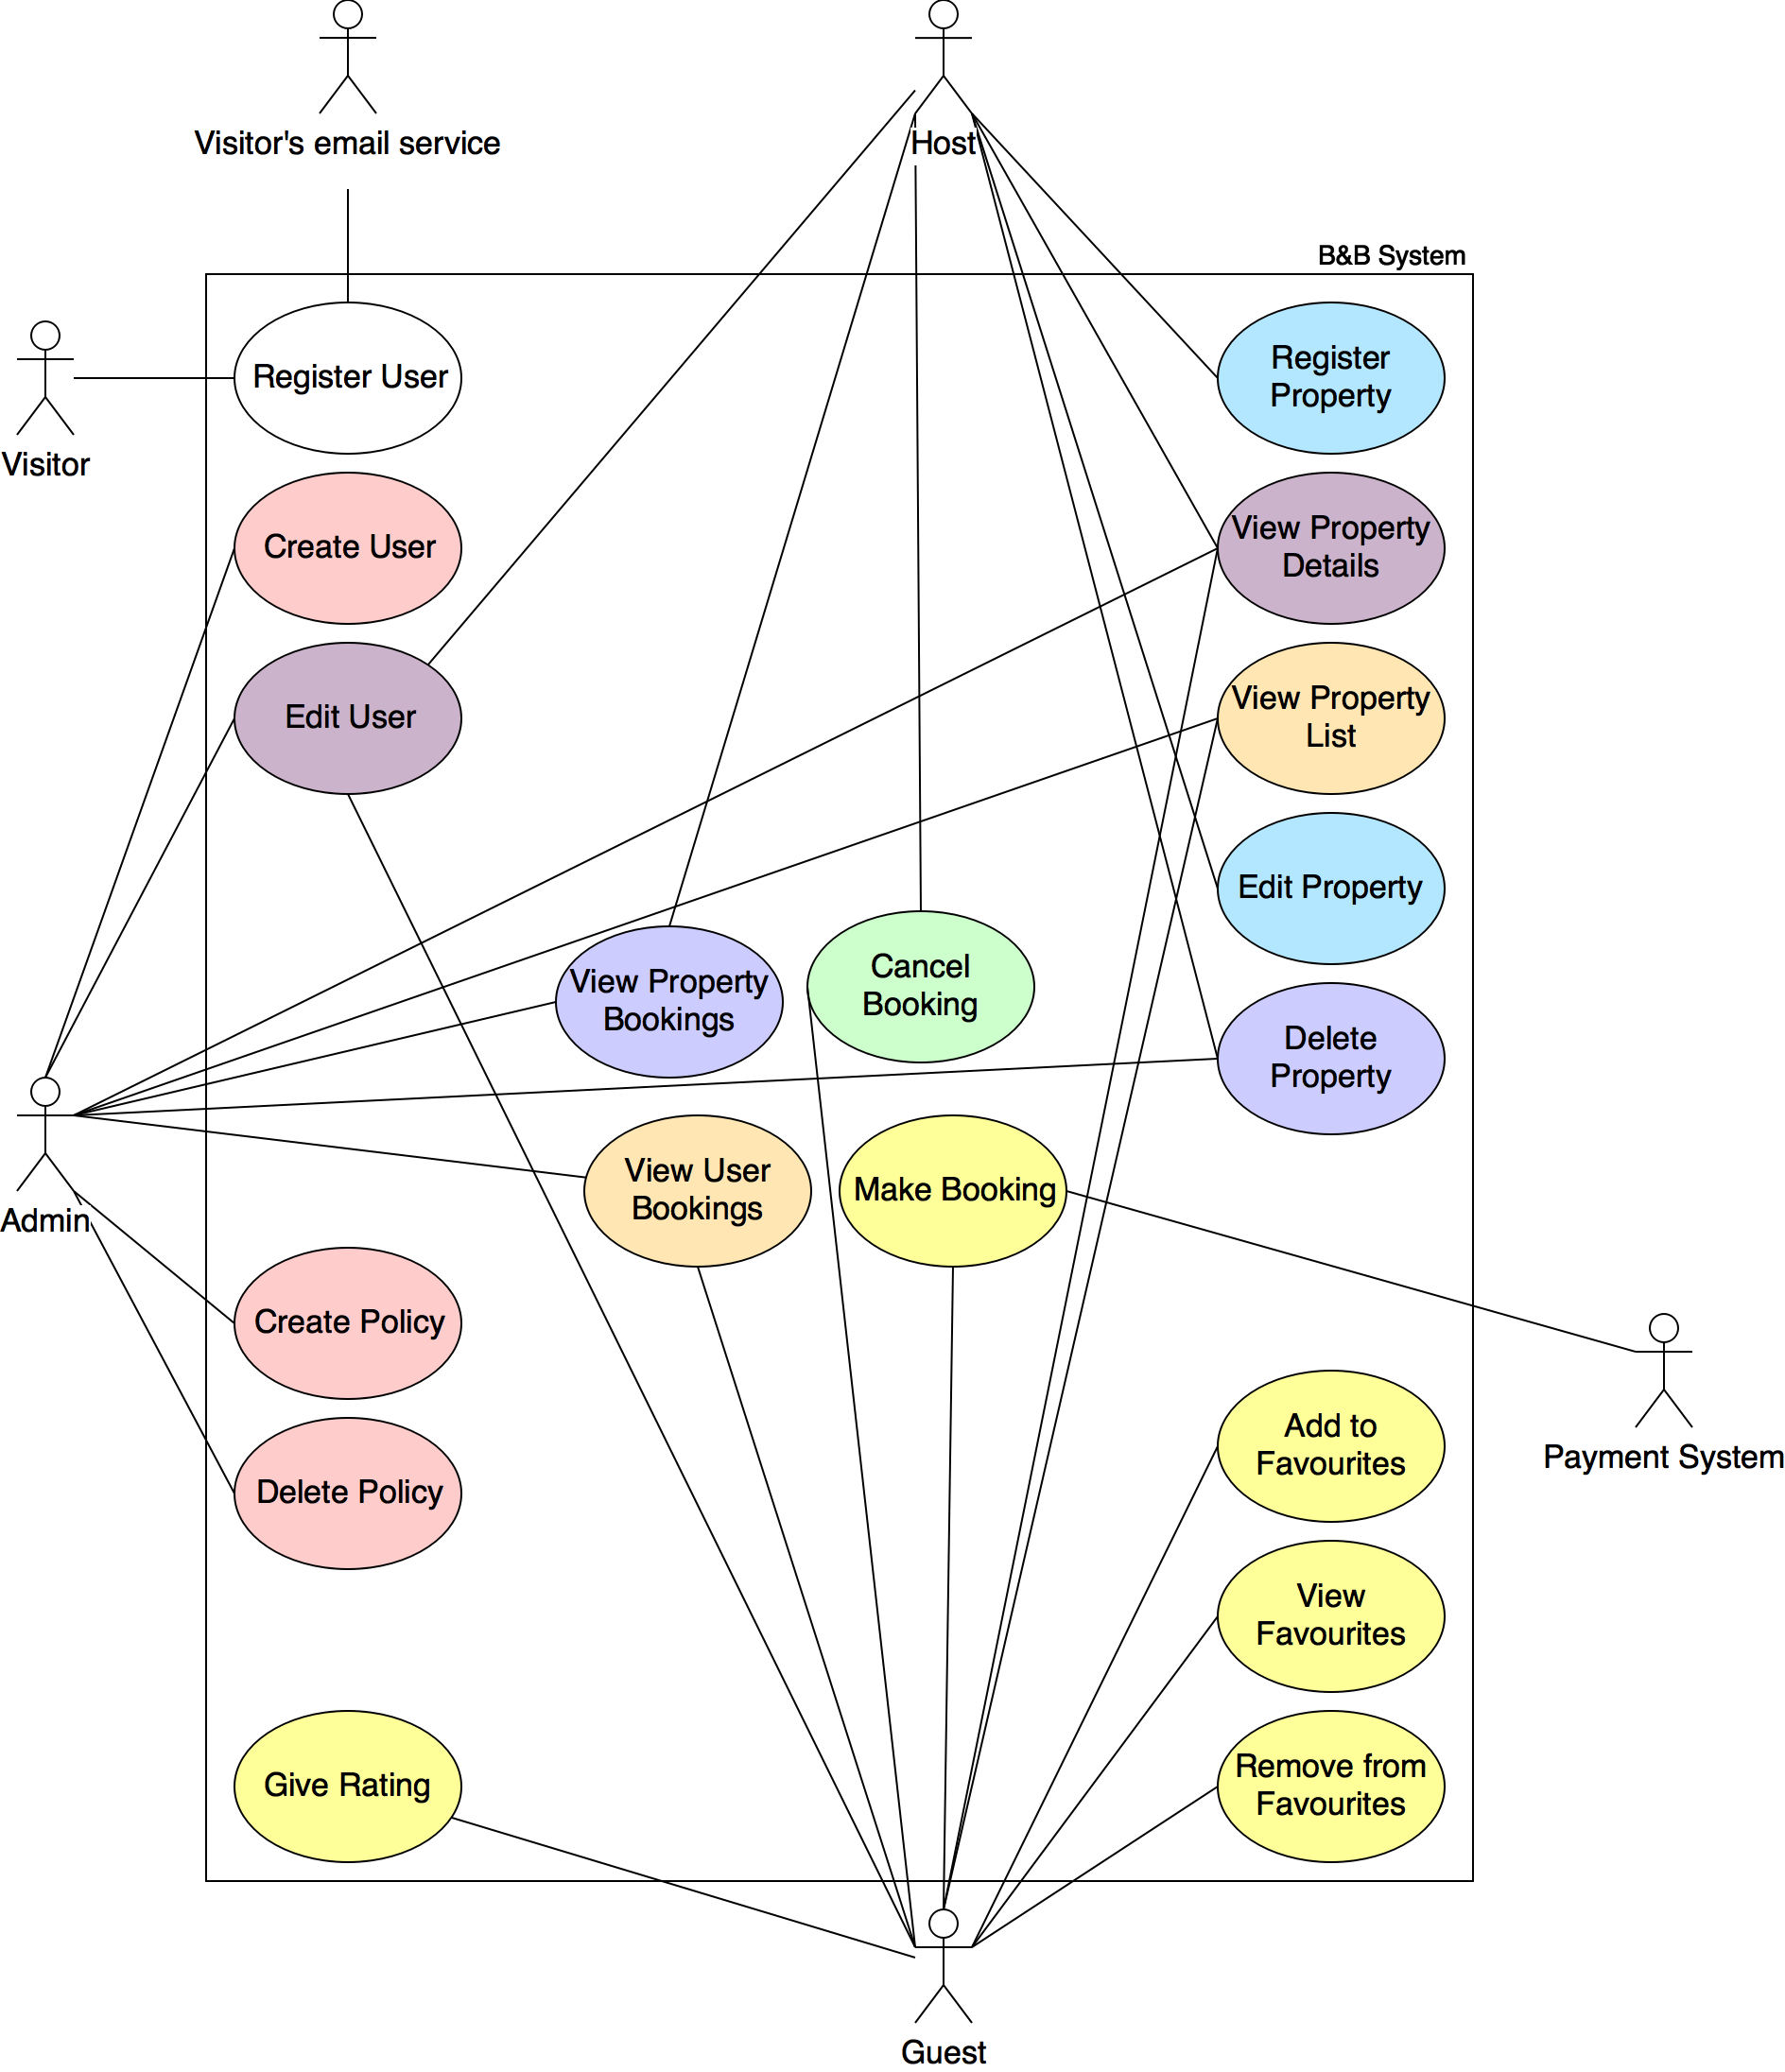
\includegraphics[width=12cm]{img/use_cases.png} \\[0.5em]
    \caption{Use Case Diagram}
    \label{use-cases-diagram}
\end{figure} 

\vspace{-1cm}
As can be seen, our set of use cases does not feature any inclusions or extensions. Strictly speaking, some of the cases do flow into each other in a way that could be thought of as extension (Make Booking, for instance, is always preceded by View Property Details). We decided not to use extensions and to include this information in the preconditions for the use cases instead, thus reducing the complexity of this representation of our system.

It can also be seen that some CRUD-like operations on the main entities were not included as full use cases (viewing/listing Users being one example). The System does, in fact, support many of these operations, but we decided to limit our list of use cases to operations that could reasonably be thought of as complete usage scenarios for a BNB Booking System. So, for instance, an Admin does have the ability to view a list of all the users on the System, but would rarely do so without, say, editing some User's details or viewing some User's Bookings afterwards.
    
We turn now to textual descriptions of the use cases. These have been written in a fair amount of detail; to condense the presentation here, we run through only the most crucial use cases. The rest are included in Appendix \ref{appendix:use-cases} \footnote{The Appendix also includes some descriptions of how the system operates that did not qualify as full use cases as they are thought of in this report (see the discussion on this above). One example of such an operation is logging in to the System (Table \ref{use_case_s1}).}. The descriptions are grouped according to the main entity being acted upon; each remaining section of this Chapter covers one of these entities. The style of these descriptions is, for the most part, based on the discussion and examples in \cite{Cockburn1998}, \cite{Blain2007} and \cite{TemplateLab}. Some more things to note:

\vspace{-0.3cm}
\begin{itemize}
    \item We have included special notation for indicating the steps at which a use case ends/can end:
    \begin{itemize}
        \item Whenever reaching a specific step means that the use case is definitely finished, the step description is preceded by "(END)".
        \item If a use case could end with some specific step, but the primary actor may still optionally perform some actions after the step in question, the step description is preceded by "(POSSIBLE END)".
    \end{itemize}  
    \item Branching is generally indicated by listing the different progression options after different letters (a, b, c...) (This is as opposed to steps that compose sequences of actions; such steps are preceded by numerals --- Arabic in the case of Main Flow steps; Roman in the case of substeps to Main Flow steps.)
    \item The flow steps generally follow the typical dialogue pattern ("The User... The System...") However, when a single actor performs multiple consecutive actions that are different enough in nature, these have been assigned their own steps to increase clarity and readability.
    \item Many of the finer details of what information is being supplied and checked at each step have been relegated to Appendix \ref{appendix:glossary} (the Glossary). As noted before the terms that are included in the glossary have been capitalized throughout the report.
    \item Whenever the Primary Actor supplies and submits some set of details to the System, and the System has the Actor resupply said details for any reason, we implicitly assume that the System saves the submitted details and displays them to the Actor when the Actor has to resupply them (so an incorrectly filled form, say, will be returned to the User with the previously submitted information already filled in).
    \item We have omitted descriptions of most confirmation messages.
    \item Some error flows have been included. However, more serious errors that should not occur during the normal operation of the System (database insertion failure, for instance) have not been individually described here for the sake of brevity. Whenever the System detects such an error, the use case being carried out stops, and the System displays an error page.
\end{itemize}

\vspace{-0.7cm}
\section{Users}
\label{use-cases-users}

For Users, we have included two creation use cases and one editing use case. The first creation case, U-C-1 (Table \ref{use_case_u-c-1}), is special in that it is the only use case with Visitor as the Main Actor. We decided that for simplicity a Visitor must first register as a Guest or a Host before gaining access to any of the real functionality of the System. The second creation case, U-C-2 (Table \ref{use_case_u-c-2} in Appendix \ref{appendix:use-cases}), is a special Admin tool, mainly meant to be used for creating more Admins. U-E (Table \ref{use_case_u-e} in Appendix \ref{appendix:use-cases}), for editing one's User Details, has a very similar flow to U-C-2. 

\begin{table}[H]
    \centering
    \footnotesize
    \begin{tabular}{| p{3.5cm} | p{12cm}@\qquad |}
      \hline
      ID & U-C-1 \\ \hline
      Use case & Register User \\ \hline
      Description & A Visitor registers as a Guest or a Host (henceforth, the Guest/Host will be referred to as "User").\\ \hline
      Primary Actor & Visitor \\ \hline
      Secondary Actor(s) & Visitor's email service \\ \hline
      Preconditions & None \\ \hline
      Main Flow &
      \vspace{-0.4cm}
        \begin{enumerate}
            \item The use case starts when the Visitor issues a request to register as a new User. 

            \item The System provides the Visitor with a means to fill in their Core User Details and Role.
            \item \label{u-c-1-cancel-fork}
            \begin{enumerate}
                \item \label{u-c-1-no-cancel}If the Visitor provides their Core User Details and Role: go to \ref{u-c-1-submit}.
                \item \label{u-c-1-cancel} If the Visitor cancels the operation: go to \ref{u-c-1-end}.
            \end{enumerate}

            \item \label{u-c-1-submit} The Visitor submits the information provided.

            \item \label{u-c-1-correct-fork} The System checks the Core User Details.
            \begin{enumerate}
                \item If the Core User Details are Correct:
                \begin{enumerate}
                    \item The System creates a new Unverified User based on the details provided.
                    \item The System sends a verification email to the email address in the Core User Details. Go to \ref{u-c-1-end}.
                \end{enumerate}
            \item \label{u-c-1-incorrect-details} If the Core User Details are not Correct: the System displays a notification about the details causing the problem. Return to 2.
            \end{enumerate}

            \item\label{u-c-1-end} (POSSIBLE END) The System displays the Landing Page.

            \item If \ref{u-c-1-cancel-fork}\ref{u-c-1-no-cancel}. taken: \label{u-c-1-verify-fork}
            \begin{enumerate}
                \item \label{u-c-1-verify} If the Visitor confirms their registration via their email service:
                \begin{enumerate}
                    \item The System changes the Unverified User into a Verified User, unlocking their account.
                    \item (END) The System confirms the verification to the User and displays the Landing Page.
                \end{enumerate}
                \item \label{u-c-1-no-verify} (END) If the Visitor never verifies their account, it remains Unverified and hence unusable.
            \end{enumerate}
            \vspace{-0.4cm}
        \end{enumerate}
         \\ \hline
        Postconditions &
        The System displays the Landing Page and:
        \begin{itemize}
            \item If \ref{u-c-1-cancel-fork}\ref{u-c-1-no-cancel}. and \ref{u-c-1-verify-fork}\ref{u-c-1-verify} taken: a new Verified User has been created; the User details correspond to those specified during the registration process. The User may begin using Guest/Host services.
            \item If \ref{u-c-1-cancel-fork}\ref{u-c-1-no-cancel}. and \ref{u-c-1-verify-fork}\ref{u-c-1-no-verify}. taken: a new Unverified User has been created; the User details correspond to those specified during the registration process. The Visitor may not access Guest/Host services until the User is Verified.
            \vspace{-0.4cm}
        \end{itemize}
        \\ \hline
    \end{tabular}
    \caption{Use Case U-C-1: Register User}
    \label{use_case_u-c-1}
  \end{table}

  \vspace{-1cm}
  Other User-related operations: the System does allow listing Users (Admin only; Requirement R-U-L-1) and viewing an individual User's User Details (Admin/Guest/Host; Requirements R-U-V-1 and R-U-V-2). These operations were not considered significant enough to warrant their own use cases. Listing is included, in effect, in all of the Admin's User-oriented use cases (in the form of the Admin's Dashboard). Viewing User Details is included in U-E. We decided that for auditing purposes, deleting Users from the system entirely would be undesirable; the Admin can instead ban misbehaving Users by editing their Details (thereby rendering them unable to do anything on the System). Logging in and logging out are described in Appendix \ref{appendix:use-cases}.

  \vspace{-0.6cm}
\section{Properties}

For Properties, we have a full set of CRUD-like use cases. We decided that viewing an individual Property's Details (P-V; Table \ref{use_case_p-v}) and the listing of Properties (including searching, filtering and sorting) (P-L; Table \ref{use_case_p-l}) were both significant enough to have their own Use Cases (a User may simply wish to check what Properties there are in a particular area for future reference, for instance). The use cases for editing and deleting a Property are in Appendix \ref{appendix:use-cases}. (Note that deleting Properties is intended to be a "soft"/"logical" delete: records and details are to be kept on the System.)

It may be worth pointing out that in P-C (Table \ref{use_case_b-c}) the Core Property Details the Host has to specify include the Rooms the Property has, and all Policies associated with those Rooms. The use case does not go into the specifics of how the Host provides these entity details, but our activity diagram covering a new Host's entire registration process (Figure \ref{activity_diagram_1} in Chapter \ref{chapter:chapter4}) includes some more information (see also Figure \ref{Sequence Diagram: Register Property} in Chapter \ref{chapter:chapter4} for the related sequence diagram.) 

\vspace{-0.2cm}
\begin{table}[H]
    \centering
    \footnotesize
    \begin{tabular}{| h | p{12cm}@\qquad |}
      \hline
      ID & P-C \\ \hline
      Use case & Register Property \\ \hline
      Description & A Host registers a new Property.\\ \hline
      Primary Actor & Host \\ \hline
      Secondary Actor(s) & None \\ \hline
      Preconditions & The Host does not already have a Property registered on their account.
      \\ \hline
      Main Flow &
      \vspace{-0.3cm}
        \begin{enumerate}
            \item The use case starts when the Host issues a request to register a Property. 
            \item The System provides the Host with a means to fill in the Core Property Details for the new Property.
            \item \label{p-c-host-fork}
            \begin{enumerate}
                \item \label{p-c-no-cancel}If the Host provides the Core Property Details: go to \ref{p-c-submit}.
                \item \label{p-c-cancel} (END) If the Host cancels the operation: the System displays the Host Dashboard.
            \end{enumerate}
            \item \label{p-c-submit} The Host submits the Core Property Details.
            \item \label{p-c-property-fork} The System checks the Core Property Details.
            \begin{enumerate}
                \item \label{p-c-correct-details}If the Core Property Details are Correct: the System creates a new Property based on the details provided.
                \item \label{p-c-incorrect-details} If the Core Property Details are not Correct: the System displays a notification about the details causing the problem. Return to 2.
            \end{enumerate}
            \item (END) The System displays the Property Details for the new Property.
            \vspace{-0.4cm}
        \end{enumerate}
        \\ \hline
        Postconditions &
        \vspace{-0.3cm}
        \begin{itemize}
            \item If \ref{p-c-host-fork}\ref{p-c-no-cancel}. and \ref{p-c-property-fork}\ref{p-c-correct-details}. taken: a Property has been created. The Core Property Details correspond to those specified during the creation process. The System displays the Property Details for the new Property.
            \item If \ref{p-c-host-fork}\ref{p-c-cancel}. taken: the System displays the Host Dashboard.
            \vspace{-0.4cm}
        \end{itemize}
         \\ \hline
    \end{tabular}
    \caption{Use Case P-C: Register Property}
    \label{use_case_p-c}
  \end{table}

  \newgeometry{left=2.3cm,bottom=0cm}
  \begin{table}[H]
    \centering
    \footnotesize
    \begin{tabular}{| w | p{12cm}@\qquad |}
      \hline
      ID & P-L \\ \hline
      Use case & View Property List \\ \hline
      Description & A Guest or an Admin (henceforth, "the User") searches for, filters, orders, and views a List of Properties.\\ \hline
      Primary Actor & Guest/Admin \\ \hline
      Secondary Actor(s) & None \\ \hline
      Preconditions & None
      \\ \hline
      Main Flow &
      \vspace{-0.3cm}
        \begin{enumerate}
            \item The use case starts when the User specifies some initial Property Search Conditions and issues a request to view a Property List. 
            \item (POSSIBLE END) The System fetches a List of Properties conforming to the Property Search Conditions set and ordered according to any Property Sort Criteria set. It also provides the User with a means to apply a new set of Property Search Conditions and to order the List according to some Property Sort Criteria. Additionally:
            \begin{enumerate}
                \item If the List is non-empty: the System displays the List and provides the User with a means to access the Property Details for each Property listed.
                \item If the List is empty: the System displays a notification informing the User that the search has produced no results.
            \end{enumerate}
            \item If the User applies a new set of Property Search Conditions and Property Sort Criteria and requests to view a new Property List: return to 2.
            \vspace{-0.8cm}
        \end{enumerate}
        \\ \hline
        Postconditions &
            The System displays a Property List conforming to the set Property Search Conditions, and ordered according to the set Property Sort Criteria.
         \\ \hline
    \end{tabular}
    \caption{Use Case P-L: View Property List}
    \label{use_case_p-l}
  \end{table}

\vspace{-0.8cm}

\begin{table}[H]
    \centering
    \footnotesize
    \begin{tabular}{| q | p{12cm}@\qquad |}
      \hline
      ID & P-V \\ \hline
      Use case & View Property Details \\ \hline
      Description & A Guest, Admin, or a Host (henceforth, "the User") views a Property's Property Details.\\ \hline
      Primary Actor & Guest/Admin/Host \\ \hline
      Secondary Actor(s) & None \\ \hline
      \vspace{-0.3cm}
      Preconditions &
      \vspace{-0.3cm}
      \begin{itemize}
        \item Admin/Guest: The Admin/Guest is viewing a Property List.
        \item Host: None.
        \vspace{-0.4cm}
    \end{itemize}
      \\ \hline
      Main Flow &
      \vspace{-0.3cm}
        \begin{enumerate}
            \item The use case starts when the User issues a request to view a Property's Property Details.
            \item (END) The System displays these Property Details. Additionally:
            \begin{enumerate}
                \item For Guest: the System provides a means to select the Initial Booking Details for a new Booking; these are pre-selected if the Guest already provided these details in some Property Search Conditions in the Precondition.
                \item For Host: the System displays the Host-Specific Property Details, and provides a means to edit the Core Property Details.
            \end{enumerate}
            \vspace{-0.4cm}
        \end{enumerate}
        \\ \hline
        Postconditions &
         The System displays the selected Property's Property Details and:
        \begin{itemize}
            \item For Guest: the System provides a means to select the Initial Booking Details for a new Booking; these are pre-selected if the Guest already provided these details in some Property Search Conditions in the Precondition.
            \item For Host: the System displays the Host-Specific Property Details, and provides a means to edit the Core Property Details.
            \vspace{-0.4cm}
        \end{itemize}
         \\ \hline
    \end{tabular}
    \caption{Use Case P-V: View Property Details}
    \label{use_case_p-v}
  \end{table}

  \restoregeometry

\section{Bookings}

Make Booking (B-C; Table \ref{use_case_b-c}) is probably the most crucial use case in the entire System. It in effect extends P-V (which, in turn, extends P-L for the Guest and Admin); the relevant postconditions from P-V are included in the preconditions for convenience.

\vspace{-0.3cm}
\begin{table}[H]
    \centering
    \footnotesize
    \begin{tabular}{| g | p{12cm}@\qquad |}
      \hline
      ID & B-C \\ \hline
      Use case & Make Booking \\ \hline
      Description & The Guest makes a new Booking.\\ \hline
      Primary Actor & Guest \\ \hline
      Secondary Actor(s) & Payment System \\ \hline
      Preconditions &
      The Guest is viewing the Property Details for a Property. The System has provided a means to select the Initial Booking Details for a new Booking; these are pre-selected if the Guest has already provided these details in some Property Search Conditions. The System has limited the Initial Booking Details the Guest may select to match the Property's availability data.
      \\ \hline
      Main Flow &
      \vspace{-0.3cm} 
        \begin{enumerate}
            \item \label{b-c-start}The use case starts when the Guest begins selecting the Initial Booking Details.
            \begin{enumerate}
                \item If the Guest selects the Initial Booking Details, or leaves them unchanged: go to \ref{b-c-submit-initial}.
                \item \label{b-c-start-cancel}(END) If the Guest cancels the operation: the System displays a Property List conforming to any Property Search Conditions and/or Property Sort Criteria set previously.
            \end{enumerate}
            \item \label{b-c-submit-initial} The Guest submits the Initial Booking Details.
            \item \label{b-c-system-booking-check}The System checks the Initial Booking Details.
            \begin{enumerate}
                \item If the Initial Booking Details are Possible: the System Locks the Initial Booking Details. Go to \ref{b-c-guest-details-form-fork}.
                \item If the Initial Booking Details are not Possible: the System displays a notification about the details causing the problem. Return to \ref{b-c-start}.
            \end{enumerate}  
            \item \label{b-c-guest-details-form-fork} The System provides the Guest with a means to fill in the full Booking Details.
            \item
            \begin{enumerate}
                \item If the Guest fills in the Booking Details: go to \ref{b-c-submit}.
                \item \label{b-c-guest-details-form-fork-cancel}(END) If the Guest cancels the operation: the System unLocks the Initial Booking Details and displays the Property Details as in the Preconditions.
            \end{enumerate}            
            \item \label{b-c-submit} The Guest submits the Booking Details.
            \item \label{b-c-check-fork} The System checks the Booking Details.
            \begin{enumerate}
                \item If the Booking Details are Correct: go to \ref{b-c-payment}.
                \item If the Booking Details are not Correct: the System displays a notification about the details causing the problem. Return to \ref{b-c-guest-details-form-fork}.
            \end{enumerate}        
            \item \label{b-c-payment} The System sends the Payment Details to the Payment System.
            \item The Payment System checks the Payment Details and sends the results back to the System.
            \item
                \begin{enumerate}
                    \item If the Payment System confirmed the Payment: 
                    \begin{enumerate}
                        \item The System unLocks the Initial Booking Details.
                        \item The System creates a Booking based on the details provided.
                        \item The System sends a confirmation email that includes the Core Booking Details to the Guest and to the Host whose Property the Booking is for. Go to \ref{b-c-end}.
                    \end{enumerate}
                    \item If not: the System displays a notification about the failed Payment. Return to \ref{b-c-guest-details-form-fork}.
                \end{enumerate}
            \item \label{b-c-end} (END) The System displays a Booking confirmation and shows the Guest's User Bookings. 
            \vspace{-0.4cm} 
        \end{enumerate} 
        \\ \hline
    \end{tabular}
    \caption{Use Case B-C: Make Booking}
    \label{use_case_b-c}
  \end{table}

  \begin{table}[H]
    \centering
    \footnotesize
    \begin{tabular}{| g | p{12cm}@\qquad |}
        \hline
        \vspace{-0.3cm} 
        Postconditions &
        \begin{itemize}
            \item If \ref{b-c-end} reached: a Booking has been created, and a Payment has been made. The Booking Details correspond to those specified during the creation process. The Guest and the Host whose Property the Booking is for have both been sent a confirmation email that includes the Core Booking Details. The System displays the User Booking List.
            \item If \ref{b-c-start}\ref{b-c-start-cancel}. taken: the System displays a Property List conforming to any Property Search Conditions and/or Property Sort Criteria set previously.
            \item If \ref{b-c-guest-details-form-fork}\ref{b-c-guest-details-form-fork-cancel}. taken: the System displays the Property Details as in the Preconditions.
        \end{itemize}
         \\ \hline
    \end{tabular}
    \caption{Use Case B-C: Make Booking (continued)}
    \label{use_case_b-c_cont}
\end{table}

We have two use cases for listing Bookings --- View User Bookings (B-L-1; Table \ref{use_case_B-L-1}) for Guests and Admins, and View Property Bookings (B-L-2; Table \ref{use_case_B-L-2}) for Hosts and Admins. These are closely analogous, so the latter has been relegated to Appendix \ref{appendix:use-cases}.

  \begin{table}[H]
    \centering
    \footnotesize
    \begin{tabular}{| w | p{12cm}@\qquad |}
      \hline
      ID & B-L-1 \\ \hline
      Use case & View User Bookings \\ \hline
      Description & A Guest views their own Bookings, or an Admin views any Guest's Bookings. (Henceforth, we will refer to the Primary Actor as "User", and to the User whose bookings are being accessed as "Target User".)\\ \hline
      Primary Actor & Guest/Admin \\ \hline
      Secondary Actor(s) & None \\ \hline
      Preconditions &
      \begin{itemize}
        \item Guest: None
        \item Admin: The Admin is viewing their Dashboard.
      \end{itemize}
      \\ \hline
      Main Flow &
        \begin{enumerate}
            \item The use case starts when the User issues a request to view the Target User's Bookings. The User Bookings are in Future mode by default.
            \item  \label{b-l-1-list} (POSSIBLE END) The System checks whether the User Bookings are in Future mode or Past mode, and:
            \begin{enumerate}
                \item If the User Bookings are in Future mode: The System displays all of the Target User's Future Bookings and provides the User a means to switch to Past mode.
                \item If the User Bookings are in Past mode: The System displays all of the Target User's Past Bookings and provides the User a means to switch to Future mode.
            \end{enumerate}
            \item If the User switches the User Bookings mode: return to \ref{b-l-1-list}.
        \end{enumerate}
        \\ \hline
        Postconditions & The System displays either the Target User's Past Bookings or the Target User's Future Bookings. (These might be empty lists.)
         \\ \hline
    \end{tabular}
    \caption{Use Case B-L-1: View User Bookings}
    \label{use_case_B-L-1}
  \end{table}

  For the following, note that Bookings are never actually deleted (from the System database) --- they are instead flagged as Cancelled Bookings and kept on the System for auditing purposes. Note also that the Payment System is not a Secondary Actor here: while it does receive the refund request, it never actually performs any actions.

  \begin{table}[H]
      \centering
      \footnotesize
      \begin{tabular}{| x | p{12cm}@\qquad |}
        \hline
        ID & B-D \\ \hline
        Use case & Cancel Booking \\ \hline
        Description & A Guest cancels one of their own Cancellable Bookings or a Host cancels a Cancellable Booking on their Property. (Henceforth, we will refer to the Primary Actor as "User".)\\ \hline
        Primary Actor & Guest/Host \\ \hline
        Secondary Actor(s) & None \\ \hline
        Preconditions & 
        \begin{itemize}
            \item Guest: The Guest is viewing their Future User Bookings.
            \item Host: The Host is viewing their Property's Future Property Bookings.
          \end{itemize}
        \\ \hline
        Main Flow &
            \begin{enumerate}
                \item The use case starts when the User requests to cancel a Booking.
                \item \label{b-d-cancellable-fork}The System checks if the Booking is Cancellable.
                \begin{enumerate}
                    \item \label{b-d-cancellable} If the Booking is Cancellable: go to \ref{b-d-confirmation-fork}.
                    \item \label{b-d-not-cancellable} If the Booking is not Cancellable: the System notifies the User that the Booking may not be cancelled. Go to \ref{b-d-end}.
                \end{enumerate}
                \item The System asks the User for confirmation.
                \item \label{b-d-confirmation-fork}
                \begin{enumerate}
                    \item \label{b-d-confirm}If the User confirms the cancellation: go to \ref{b-d-confirmed}.
                    \item \label{b-d-cancel}If the User cancels the operation: go to \ref{b-d-end}.
                \end{enumerate}
                \item \label{b-d-confirmed} Using the Payment Details for the Bookings, the System sends a refund request to the Payment System.
                \item The System makes the Booking a Cancelled Booking.
                \item The System sends a cancellation email that includes the Core Booking Details to the Guest who made the Booking and to the Host whose Property the Booking was for.
                \item \label{b-d-end} (END) The System displays the User/Property Bookings as in the Preconditions.
          \end{enumerate}
          \\ \hline
          Postconditions &
          The System displays the User/Property Bookings as in the Preconditions and:
          \begin{itemize}
              \item If \ref{b-d-cancellable-fork}\ref{b-d-cancellable}. and \ref{b-d-confirmation-fork}\ref{b-d-confirm}. taken: the Booking is now a Cancelled Booking. The Guest who made the Booking and the Host whose Property the Booking was for have been sent a cancellation email that includes the Core Booking Details.
          \end{itemize}
           \\ \hline
      \end{tabular}
      \caption{Use Case B-D: Cancel Booking}
      \label{use_case_b-d}
  \end{table}

  \section{Policies}

  Only Admins have access to the Policy-related use cases. Only creating (Po-C; Table \ref{use_case_po-c}) and deleting (Po-D; Table \ref{use_case_po-d}) Policies were deemed important enough to qualify for their own use cases. The Admin can view a list of Policies on their Dashboard; editing Policies is not necessary since they are so simple (one would simply delete the existing Policy and create a new one in its place).

\begin{table}[H]
    \centering
    \footnotesize
    \begin{tabular}{| a | p{12cm}@\qquad |}
      \hline
      ID & Po-C \\ \hline
      Use case & Create Policy \\ \hline
      Description & An Admin creates a new Policy.\\ \hline
      Primary Actor & Admin \\ \hline
      Secondary Actor(s) & None \\ \hline
      Preconditions & The Admin is viewing their Dashboard.
      \\ \hline
      Main Flow &
        \begin{enumerate}
            \item The use case starts when the Admin issues a request to create a Policy. 
            \item The System provides the Admin with a means to fill in the Name for the new Policy.
            \item \label{po-c-admin-fork}
            \begin{enumerate}
                \item \label{po-c-no-cancel}If the Admin provides the Policy Name: go to \ref{po-c-submit}.
                \item \label{po-c-cancel} If the Admin cancels the operation: go to \ref{po-c-policy-list}.
            \end{enumerate}
            \item \label{po-c-submit} The Admin submits the Policy Name.
            \item \label{po-c-policy-fork} The System checks the Policy Name.
            \begin{enumerate}
                \item \label{po-c-success}If the Policy Name is unique: the System creates a new Policy with the Policy Name provided.
                \item \label{po-c-policy-exists} If a Policy with the same Name already exists: the System displays a notification about the potential duplication. Return to 2.
            \end{enumerate}
            \item \label{po-c-policy-list} (END) The System displays the Admin's Dashboard.
        \end{enumerate}
        \\ \hline
        Postconditions &
        The System displays the Admin's Dashboard and:
        \begin{itemize}
            \item If \ref{po-c-admin-fork}\ref{po-c-no-cancel}. and \ref{po-c-policy-fork}\ref{po-c-success}. taken: a Policy has been created. The Policy has the Policy Name specified during the creation process.
        \end{itemize}
         \\ \hline
    \end{tabular}
    \caption{Use Case Po-C: Create Policy}
    \label{use_case_po-c}
  \end{table}

  \begin{table}[H]
    \centering
    \footnotesize
    \begin{tabular}{| a | p{12cm}@\qquad |}
      \hline
      ID & Po-D \\ \hline
      Use case & Delete Policy \\ \hline
      Description & An Admin deletes a Policy.\\ \hline
      Primary Actor & Admin \\ \hline
      Secondary Actor(s) & None \\ \hline
      Preconditions & The Admin is viewing their Dashboard.
      \\ \hline
      Main Flow &
        \begin{enumerate}
            \item The use case starts when the Admin issues a request to delete a Policy.
            \item The System asks the Admin for confirmation.
            \item \label{po-d-admin-fork}
            \begin{enumerate}
                \item \label{po-d-confirm-deletion} If the Admin confirms the deletion: go to \ref{po-d-system-fork}.
                \item \label{po-d-cancel-operation} If the Admin cancels the operation: go to \ref{po-d-display-list}.
            \end{enumerate}
            \item \label{po-d-system-fork}
            The System deletes the Policy and removes it from all affected Rooms.
            \item \label{po-d-display-list} (END) The System displays the Admin's Dashboard.
        \end{enumerate}
        \\ \hline
        Postconditions &
            The System displays the Admin's Dashboard and:
            \begin{itemize}
                \item If \ref{po-d-admin-fork}\ref{po-d-confirm-deletion}. taken: the Policy has been deleted; the Policy has been removed from all affected Rooms.
            \end{itemize}
            \\ \hline
    \end{tabular}
    \caption{Use Case Po-D: Delete Policy}
    \label{use_case_po-d}
  \end{table}

\section{Ratings}

Everything to do with Ratings is handled via a single use case, R-C (Table \ref{use_case_r-c}). The Ratings are displayed as part of the Property Details in P-V, and we decided that to be sufficient (in terms of viewing/listing Ratings) for the scope of this project. One straightforward extension of the current setup would enable each Guest to see a list of all Ratings they have given and allow the Admin to see all Ratings System-wide in a single list. No special editing or deleting use cases have been included: Ratings can be replaced by rating the Property in question again.

\begin{table}[H]
    \centering
    \footnotesize
    \begin{tabular}{| g | p{12cm}@\qquad |}
      \hline
      ID & R-C \\ \hline
      Use case & Give Rating \\ \hline
      Description & A Guest gives a Rating to a Property for which they have a Past Booking.\\ \hline
      Primary Actor & Guest \\ \hline
      Secondary Actor(s) & None \\ \hline
      Preconditions & The Guest is viewing their Past User Bookings.
      \\ \hline
      Main Flow &
        \begin{enumerate}
            \item The use case starts when the Guest selects a Booking from their Past User Bookings and issues a request to give a Rating to the Property associated with that Booking. 
            \item \label{r-c-existing-rating-fork} The System checks if the Guest already has a Rating for this Property.
            \begin{enumerate}
                \item \label{r-c-no-existing-rating}If the Guest does not have a Rating for this Property: go to \ref{r-c-rating}.
                \item \label{r-c-existing-rating}If the Guest has a Rating for this Property: the System notifies the Guest that the existing Rating will be overwritten if the operation is completed. Go to \ref{r-c-rating}.
            \end{enumerate}
            \item \label{r-c-rating} The System provides the Guest with a means to fill in the Rating Details for the new Rating.
            \item \label{r-c-rating-fork}
            \begin{enumerate}
                \item \label{r-c-select} If the Guest fills in the Rating Details: go to \ref{r-c-check-fork}.
                \item \label{r-c-cancel} If the Guest cancels the operation: go to \ref{r-c-user-bookings}.
            \end{enumerate}
            \item \label{r-c-check-fork} The System checks if the Rating Details are Correct.
            \begin{enumerate}
                \item \label{r-c-check-ok} If the Rating Details are Correct:
                \begin{enumerate}
                    \item If \ref{r-c-existing-rating-fork}\ref{r-c-existing-rating}. taken: the System deletes the existing Rating. In any case:
                    \item \label{r-c-give-rating}The System creates a new Rating for this Property based on the details provided, and associates it with this Guest. Go to \ref{r-c-user-bookings}.
                \end{enumerate}
                \item If the Rating Details are not Correct: return to \ref{r-c-rating}.
            \end{enumerate}
            \item \label{r-c-user-bookings} (END) The System displays the Guest's Past User Bookings.
        \end{enumerate}
        \\ \hline
        Postconditions &
        The System displays the Guest's Past User Bookings and:
        \begin{itemize}
            \item If \ref{r-c-existing-rating-fork}\ref{r-c-existing-rating}., \ref{r-c-rating-fork}\ref{r-c-select}. and \ref{r-c-check-fork}\ref{r-c-check-ok}. taken: the existing Rating for this Property by this Guest has been deleted, and a new Rating has been created. The Rating has the Rating Details specified during the creation process. 
            \item If \ref{r-c-existing-rating-fork}\ref{r-c-no-existing-rating}., \ref{r-c-rating-fork}\ref{r-c-select}. and \ref{r-c-check-fork}\ref{r-c-check-ok}. taken: a new Rating for this Property by this Guest has been created. The Rating has the Rating Details specified during the creation process.
        \end{itemize}
         \\ \hline
    \end{tabular}
    \caption{Use Case R-C: Give Rating}
    \label{use_case_r-c}
  \end{table}

\section{Favourites}
\label{use-cases-favourites}

The Favourites are only accessible to Guests, and seeing as the entities are very simple in nature (amounting to nothing more than links between Users and Properties), no editing use case is required. Adding a Property to one's Favourites (F-C; Table \ref{use_case_f-c}) and viewing one's Favourites (F-L; Table \ref{use_case_f-l}) are featured here; removing a Property from one's Favourites (F-D; Table \ref{use_case_f-d}) is in Appendix \ref{appendix:use-cases}.

\begin{table}[H]
    \centering
    \footnotesize
    \begin{tabular}{| g | p{12cm}@\qquad |}
      \hline
      ID & F-C \\ \hline
      Use case & Add to Favourites \\ \hline
      Description & A Guest adds a Property to their Favourites.\\ \hline
      Primary Actor & Guest \\ \hline
      Secondary Actor(s) & None \\ \hline
      Preconditions & The Guest is viewing the Property Details for Property to be added.
      \\ \hline
      Main Flow &
        \begin{enumerate}
            \item The use case starts when the Guest issues a request to add the Property to their Favourites. 
            \item The System adds the Property to the Guest's Favourites.
            \item (END) The System displays the Property Details, with a symbol indicating that the Property is in the Guest's Favourites.
        \end{enumerate}
        \\ \hline
        Postconditions & The Property is added to the Guest's Favourites. The System displays the Property Details, with a symbol indicating that the Property is in the Guest's Favourites.
         \\ \hline
    \end{tabular}
    \caption{Use Case F-C: Add to Favourites}
    \label{use_case_f-c}
  \end{table}

  \begin{table}[H]
    \centering
    \footnotesize
    \begin{tabular}{| g | p{12cm}@\qquad |}
      \hline
      ID & F-L \\ \hline
      Use case & View Favourites \\ \hline
      Description & A Guest views their Favourites.\\ \hline
      Primary Actor & Guest \\ \hline
      Secondary Actor(s) & None \\ \hline
      Preconditions & None
      \\ \hline
      Main Flow &
        \begin{enumerate}
            \item The use case starts when the Guest issues a request to view their Favourites.
            \item (END) The System displays the Guest's Favourites and provides a means for the Guest to request to view the Property Details for each Property in the Favourites.
        \end{enumerate}
        \\ \hline
        Postconditions & The System displays the Guest's Favourites and provides a means for the Guest to request to view the Property Details for each Property in the Favourites.
         \\ \hline
    \end{tabular}
    \caption{Use Case F-L: View Favourites}
    \label{use_case_f-l}
  \end{table}